%%%%%%%%%%%%%%%%%%%%%%%%%%%%%%%%%%%%%%%%%%%%%%%%%%%%%%%%%%%
% --------------------------------------------------------
%  _____           
% |_   _|_ _ _   _ 
%   | |/ _` | | | |
%   | | (_| | |_| |
%   |_|\__,_|\__,_|
%
% LaTeX2e Template
% Version 2.5.0 (01/01/2026)
%
% Author: 
% Guillermo Jimenez (memo.notess1@gmail.com)
% 
% License:
% Creative Commons CC BY 4.0
% --------------------------------------------------------
%%%%%%%%%%%%%%%%%%%%%%%%%%%%%%%%%%%%%%%%%%%%%%%%%%%%%%%%%%%
% --------------------------------------------------------
% Github Repository:
% https://github.com/MemoJimenez/Tau-class
% --------------------------------------------------------
%%%%%%%%%%%%%%%%%%%%%%%%%%%%%%%%%%%%%%%%%%%%%%%%%%%%%%%%%%%


\documentclass[9pt,a4paper,twocolumn,twoside]{tau-class/tau}
\usepackage[ngerman]{babel} %if wanted ngerman
\usepackage{verbatim}
% Spanish babel recomendation
% \usepackage[spanish,es-nodecimaldot,es-noindentfirst]{babel} 

%----------------------------------------------------------
% Title & Authors/Affiliations
%----------------------------------------------------------

\doctype{Zusammenfassung der Ergebnisse der Projektarbeit}
\title{Neuronales Netz f\"ur den kalifornischen Hauspreis-Datensatz}


%----------------------------------------------------------

\author[a]{Florian Adamczyka}%\thanks{\href{mailto:author.one@institute.org}{author.one@institute.org} (A. One)}}
\author[b]{Felix Hollfoth}
\author[c]{Kolja Scriba}
\author[d]{Björn Becker}
\author[e]{Felix Neumann}
%if wantet [a,1]
%----------------------------------------------------------

\affil[a]{Justus-Liebig-Universität, Matrikelnr. 8105234}
\affil[b]{Justus Liebig Universität, Matrikelnr. 8221324}
\affil[c]{Justus Liebig Universität, Matrikelnr. 8111369}
\affil[d]{Justus Liebig Universität, Matrikelnr. 8206290}
\affil[e]{Justus Liebig Universität, Matrikelnr. 8116639}
%----------------------------------------------------------
% Document-, Footer- information
%----------------------------------------------------------

\dates{This manuscript was compiled on \today}

%\docinfo{This document class was prepared on Overleaf and compiled with pdf\LaTeX{}. No errors were found during the compilation process. Tau-class supports external editors, though additional setup may be required.} 

%----------------------------------------------------------

\dates{Gruppe 308 -- KI~I Projekt WS~2025/26}
\footinfo{KI~I Portfolio}
\theday{\today}
\organization{JLU Gießen}
%\leadauthor{F.\ Neumann}

%----------------------------------------------------------
% ABSTRACT AND KEYWORDS
%----------------------------------------------------------

\begin{abstract}    
    Dieser Ergebnisbericht dokumentiert die Ergebnisse der Gruppe 308 der Projektarbeit zu Maschinellem Lernen im Modul Künstliche Intelligenz 1. 
    Die Aufgabenstellung lautete auf dem Datensatz zu den kalifornischen Hauspreisen, wie in der Vorlesung betrachtet ein neuronales Netz, um die Hauspreise zu beschreiben zu entwickeln. 
    Im Anschluss soll dieses mit der linearen Regression verglichen werden.
    Die Bearbeitungszeit betrug pro Gruppenmitglied mindestens 75 Stunden und wurde
    in mehreren Meetings zwischen den Personen aufgeteilt. Neben der linearen Regression
    wurden auch andere Regressionsmodelle als Vergleichsgrundlage für das Neuronale Netz herangezogen. 
    Der Schwerpunkt liegt allerdings auf der sukzessiven Verbesserung des Neuronalen Netzes, unter Anwendung der Vorlesungsinhalte.
    Die Optimierung der Regression erfolgt unter ständiger Kontrolle der Fehlergrößen wie dem Mean Squared Error (=MSE) und dem Root Mean Square Error (=RMSE), sowie dem coefficient of determination ($=R^2$) als quantitativer Vergleich der Modelle.
\end{abstract}

    % Tau ($\tau$) is a specially designed document class for creating professional and well-structured research articles, technical reports, and academic documentation. Tau enhances the writing experience through intuitive custom environments, multilingual support, and refined typography powered by Fira Sans for headings and distinctive elements, Fira Modo for listings, and STIX2 for body text, providing consistent and professional styling for elements such as tables, figures, equations, code listings, and captions. \textit{New/Updated features will show a (*) in their title.}

%----------------------------------------------------------

\keywords{euronales Netz, California Housing, TensorFlow, Regression, Machine Learning}

%----------------------------------------------------------

\begin{document}
		
    \maketitle 
    \thispagestyle{firststyle}
    
%----------------------------------------------------------

\section{Explorative Datenanalyse, -Bereinigung und -Darstellung (Florian)}
\taustart{D}ie explorative Datenanalyse dient der Aufnahme von Eckdaten des Datensatzes
und dem erlangen eines Gefühls für potenzielle Besonderheiten,
die in der Datenbereinigung für ein besseres Ergebnis sinnvoll behoben werden.
    \subsection{Analyse}
        Die Explorative Datenanalyse ergab, dass zwei der acht Features des Datensatzes cut-off-Werte besitzen.
        Eine unrealistisch hohe Anzahl an Werten befindet sich hierbei genau an der Grenze der aufgetragenen Werte. 
        Zudem ist eine hohe Streuung der Werte mit einigen vermeintlichen Ausreißern direkt zu erkennen.
        Um damit überhaupt beginnen zu können, hat Florian ein Projektinfrastruktur mit git, allgemeinen Funktionen, 
        Anweisungen und den utils geschaffen, sowie die Daten eingelesen. Auf dieser Grundlage konnte dann mit der inhaltlichen Arbeit 
        begonnen werden. 
    
    \subsection{Bereinigung}
        Die Cut-Off-Werte der Features 'MedHouseVal' und 'HouseAge'  wurden mit den Outliern über dem 98\%-Quantil
        bei den Features 'AveRooms', 'AveBedrms', 'Population' und 'AveOccup' entfernt, da diese Artefakte darstellen und das Rauschen des Datensatzes erhöhen.
        Aus den ursprünglich 20.000 Datenpunkten verbleiben nach der Bereinigung noch 17.386. 

    \subsection{Skalierung}
        Zuletzt wurde der Datensatz noch in einen Test-(80\% Anteil) und Trainingsdatensatz(20\% Anteil) aufgeteilt. 
        Aus dem Testdatensatz wurde dann zum lernen der Modelle noch ein Validierungsdatensatz entnommen.
        Für das Training der Modelle mit verschiedensten Aktivierungsfunktionen ist eine Skalierung zwingend notwendig um ein sinnvolles Ergebnis zu erhalten. 
        In Notebook 0c wurde zu diesem Zweck ein Standard-Skalierer und drei Minimum-Maximum-Skalierer
        implementiert, auf die in den jeweiligen Notebooks zurück gegriffen werden wird.
    \subsection{Darstellungen bereinigter Daten}
        \figref{fig:figure_1} Datensatz mit entfernten Cut-Off-Werten und Ausreißern sortiert nach Features.
        Im Vergleich mit den Originaldaten gibt es bei den modifizierten Features keine gehäuften Datenansammlungen am Ende der Skala und keine groben Ausreißer mehr.
        \begin{figure}[H]
    		\centering
    		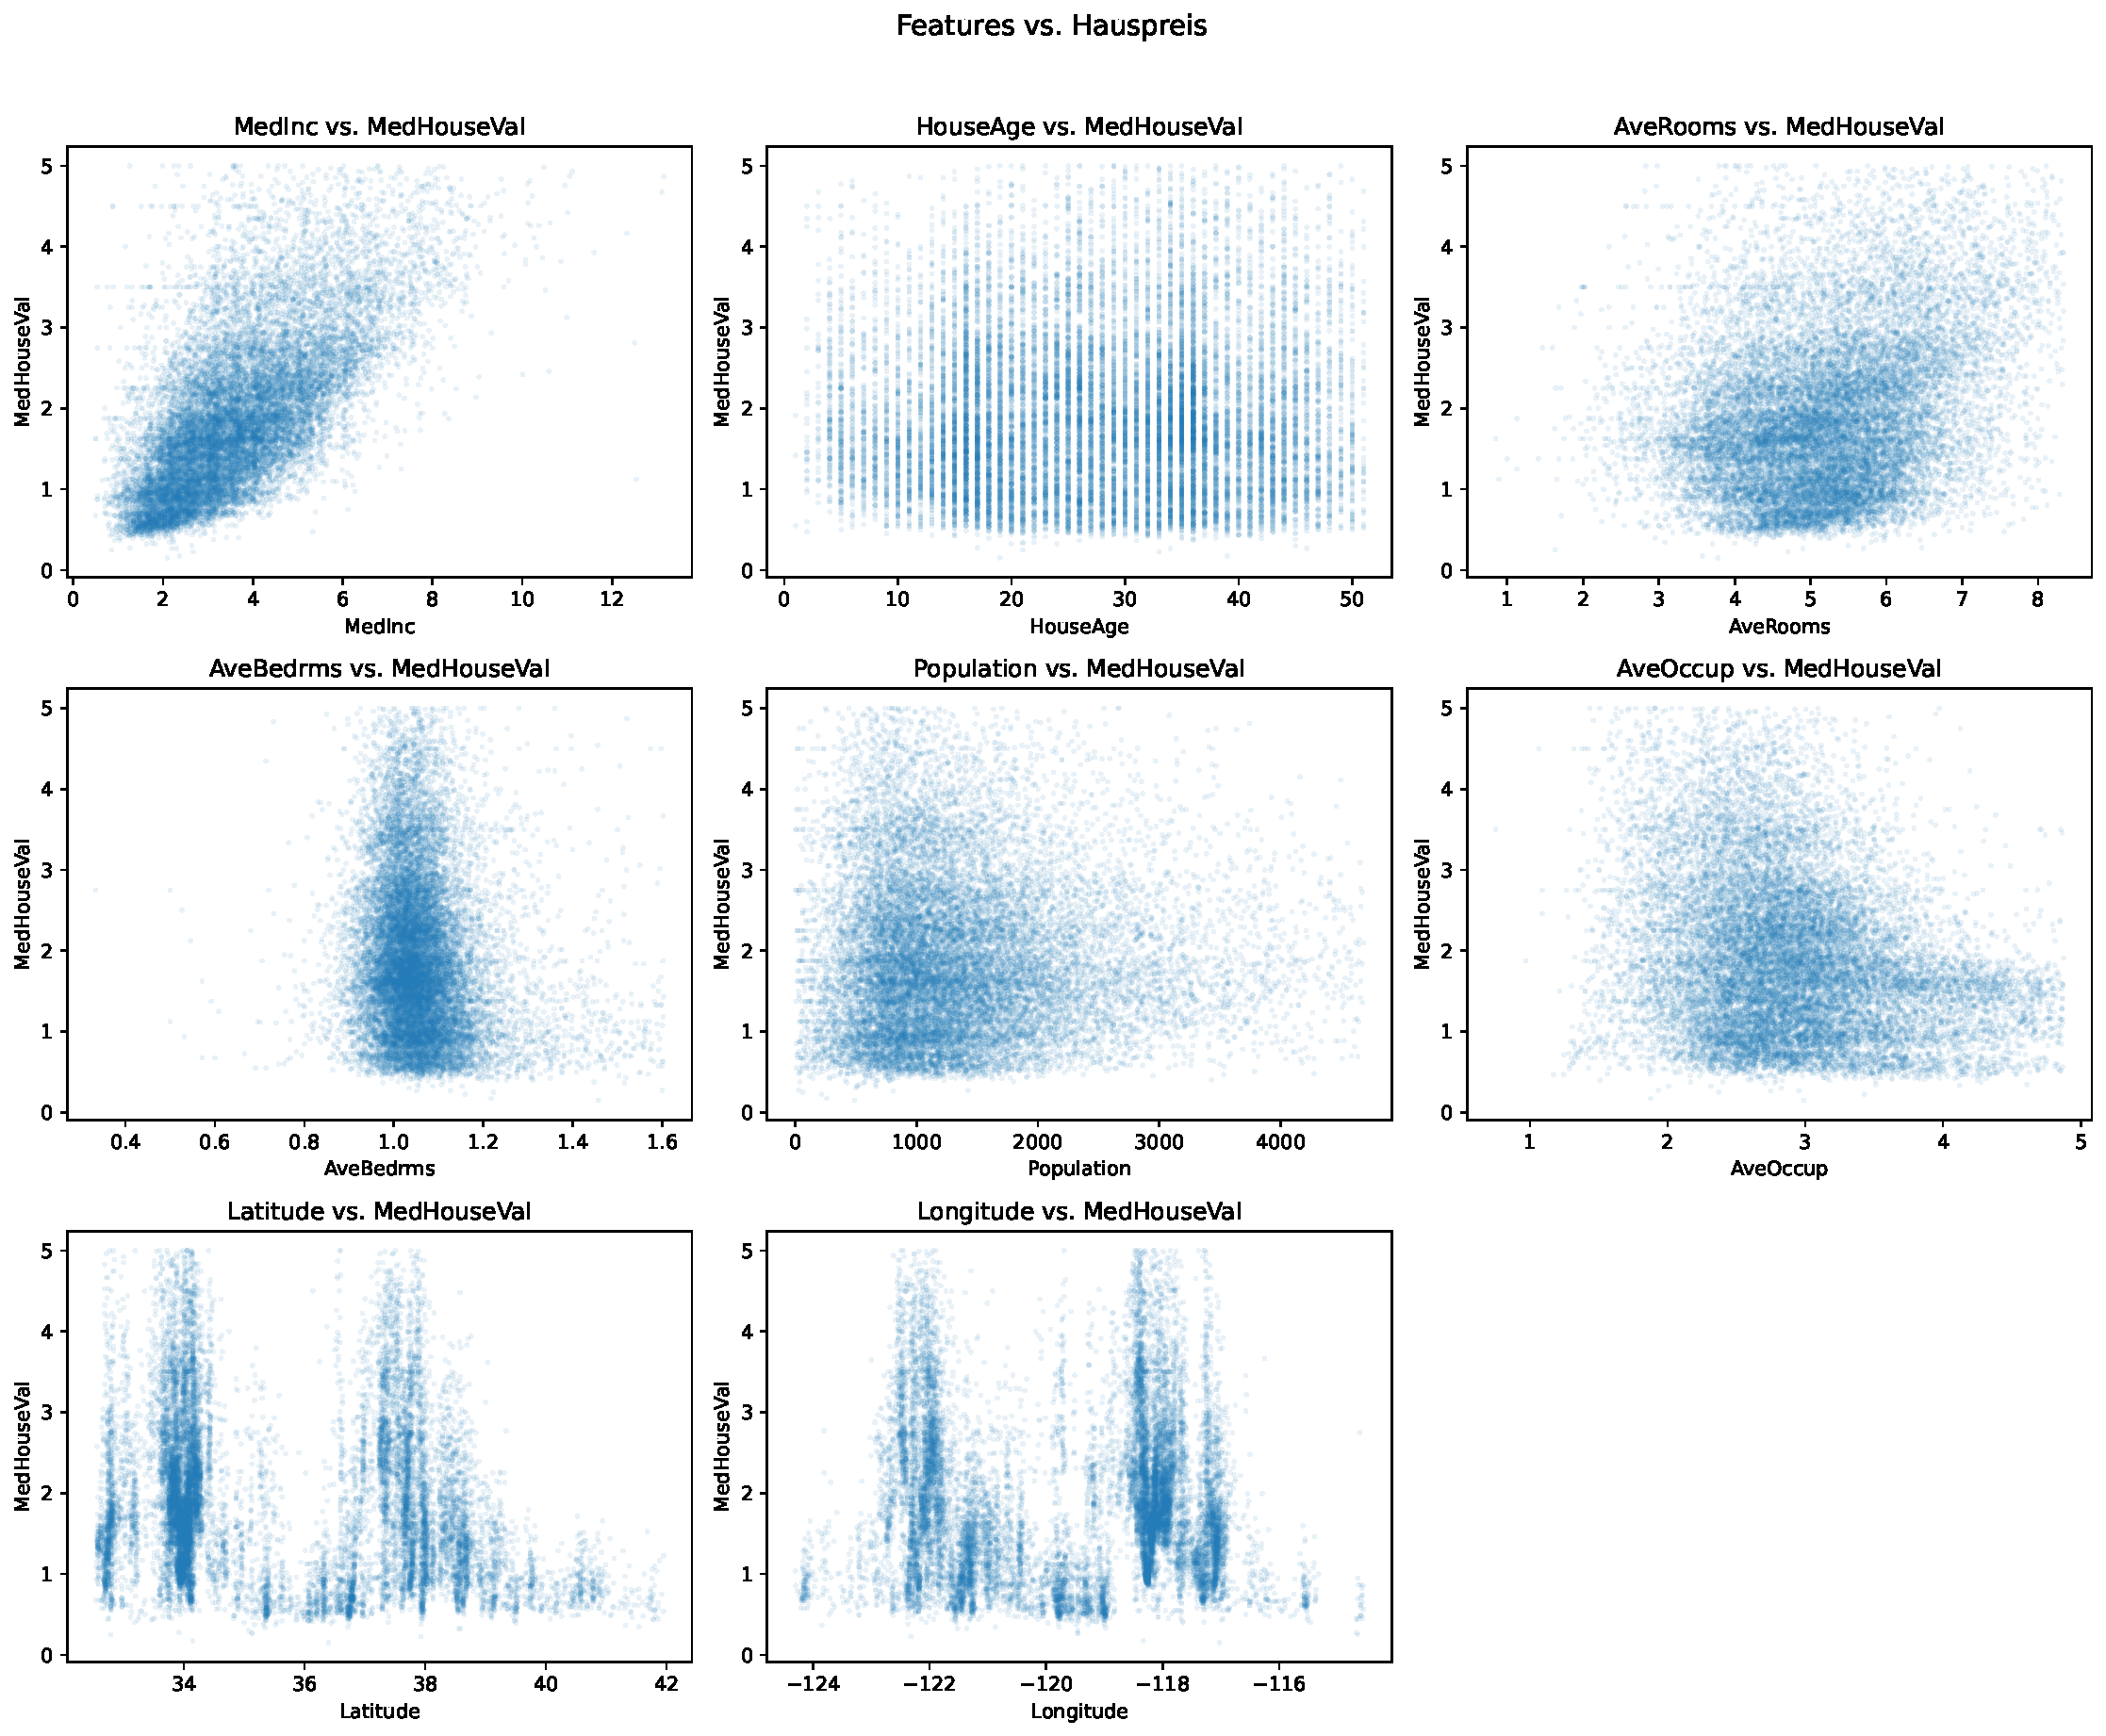
\includegraphics[width=0.75\columnwidth]{figures/eda_features_vs_target_clean.pdf}
    		\caption{Bereinigte Daten sortiert nach Features.}
    		\label{fig:figure_1}
    	\end{figure}

    	\figref{fig:figure_2} Die nach  der Datenbereinigung durchgeführte Korrelationsanalyse zeigt den starken Zusammenhang  zwischen 'MedHouseVal' und 'MedInc'.
    		
    	\begin{figure}[H]
    		\centering
    		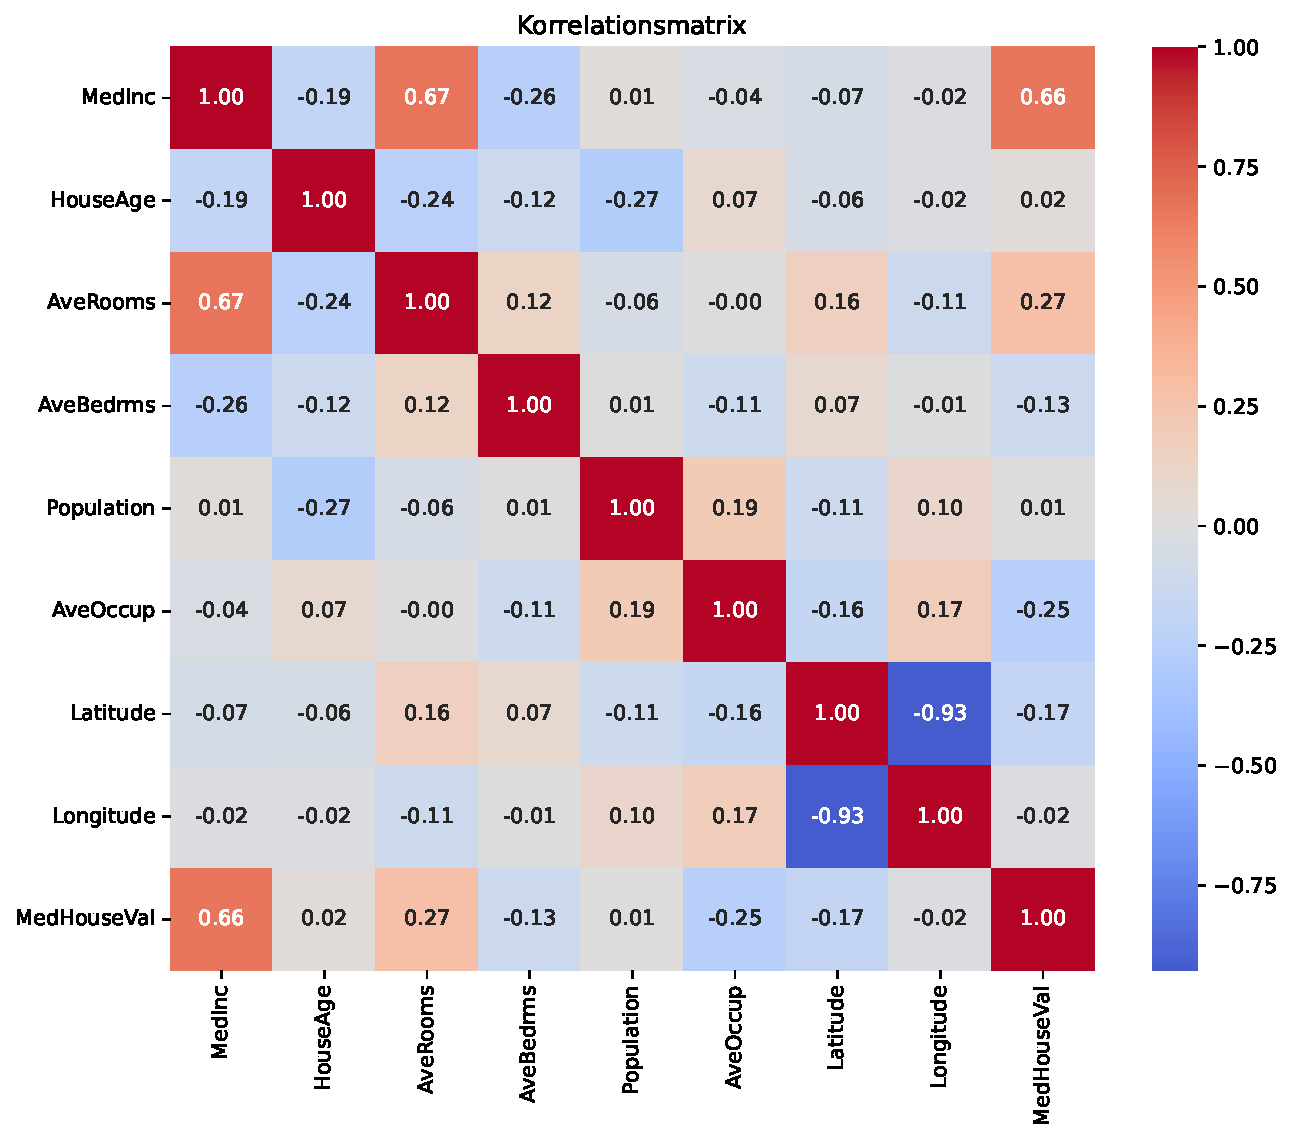
\includegraphics[width=0.75\columnwidth]{figures/eda_correlation_heatmap.pdf}
    		\caption{Korrelationsanalyse der bereinigten Daten}
    		\label{fig:figure_2}
    	\end{figure}

        


\section{Lineare Regression}
        Die als Vergleichsmodell für die Bewertung komplexerer Modelle von Florian
        implimentierte lineare Regression, erzielt unskaliert folgende Ergebnisse:

%\tabref{tab:table} shows an example table of some astronomical objects. 

        \begin{table}[H]
        	\caption{Ergebnisse der linearen Regression}
        	\label{tab:table}
        	\begin{tabular}{
        		>{\raggedright\arraybackslash}p{0.25\columnwidth}
        		>{\raggedright\arraybackslash}p{0.30\columnwidth}
        		>{\raggedright\arraybackslash}p{0.31\columnwidth}
        	}
        	\toprule
        	\textbf{Metrik} & \textbf{Train} & \textbf{Test} \\
        	\midrule
        	$R^2-Score$        & 0.6465        & 0.6326            \\
            MAE                & 0.4252        & 0.4331           \\
            RMSE               & 0.5710        & 0.5779            \\
        	\bottomrule
        	\end{tabular}
        	%\tabletext{Note: The table contains data of some famous celestial objects.}
        \end{table}

        Diese Werte stellen die "Baseline" zur Einordnung komplexerer Modelle dar
        und geben einen ersten Anhaltspunkt über die potenzielle Leistung der Regressionen.

        \subsection{LASSO und Ridge (Florian, Kolja)}
        Eine Erweiterung der linearen Regression durch eine LASSO-Ridge Kombination, sowie die Verwendung des Standard-Scaler führten zunächst zu keiner Verbesserung gegenüber der Baseline.
        Entscheidende Unterschiede zeigten sich durch die Einführung der Polynomialen Erweiterung. 
        Zunächst eine Verbesserung in der zweiten und  nochmal geringfügig in der dritten Ordnung. Am Ende konnte ein $R^2 =  0.7184 $
        auf die Testdaten erreicht werden ($\Delta_{Baseline} R^2 = 8.58\%$). 
        Durch die gewählten Methoden konnte auch ein sehr geringer Overfitting-Gap erzielt werden.

        
\section{Decision Tree Regression (Florian)}
        Ausgehend von den Vorlesungsinhalten wurden Decision Trees zunächst als Referenz ohne Einschränkungen
        und dann mit Beschränkung der maximalen Tiefe gegen Overfitting Probleme trainiert. 
        Der Overfitting-Gap bei ersterm lag bei knapp 45\%. Bei zweiterem wurde der bias-varianz-tradeoff sichtbar.
        Durch Pruning konnte das Overfitting des Baums auf die Testdaten sehr erfolgreich unterbunden werden. 
        Wie auch bei der Explorativen Datenanalyse zeigt sich, dass das Median Einkommen (=MedInc) die Featureimportance dominiert 
        (siehe \figref{fig:figure_5}). 
%%% Referenz schreiben

\section{Ensemble (Florian)}
        Die Ensemble-Methoden wurden als Test für die mögliche Genauigkeit der Regression verwendet.
        Die Ergebnisse der Decision Trees konnten als Random Forest enorm verbessert werden. 
        Auch die Verwendung des Gradient Boosting und die Optimierung der learning rate konnten bessere Regressionen liefern. 
        Diese Erkenntnis und ein maximales $R^2 = 0.81$ ($\Delta_{Baseline} R^2 = 17.74\%$), als Marker für die mögliche Leistung der Regression,
        wurden in das Training neuronaler Netze einbezogen.


\section{K-Nearest Neighbors Regression (Florian)}
        Die K-Nearest Neighbors Regression hingegen zeigte keine allzu zuverlässigen Ergebnisse. Sie zeigte jedoch auf,
        wie unerlässlich eine Skalierung der Daten sein kann. Eine gleichzeitige Reduktion zweier Fehlerquellen führt zum bias-variance-tradeoff bei der Wahl
        des besten k. Durch Distance weighting wurde eine Verbesserung erzielt, allerdings rechtfertigen die Ergebnisse ($\Delta_{Baseline} R^2 \approx 3.01\%$)
        die viel längere Rechenzeit nicht.


\section{Neuronale Netze}
        Verschiedene Neuronale Netze (=NN) wurden, ausgehend von einem sequenziellen Netz mit einem Hidden Layer (=HL) als Minimalnetz,
        zunächst ohne optimierte Parametrisierung, ausprobiert. Bereits bei diesem Minimalnetz ergab sich ($\Delta_{Baseline} R^2 \approx 10\%$).
        Im Anschluss testeten wir verschiedene Optimierungsansätze: 
        \subsection{Architektur}
        Durch eine geschickte Wahl oder bewusstes Freistellen der Wahl der Parameter des Aufbaus des neuronalen Netzes wurden kleine Verbesserungen
        der Regression erreicht.
            \subsubsection{Layer (Björn, Felix H., Felix N., Florian; Kolja)}
            Die Variation der Breite und Layer ergab keine großen Veränderungen für das Neuronale Netz. Ein zu schmaler Layer vermag die
            komplexen Zusammenhänge zwischen einzelnen Merkmalen nicht ausreichend zu beschreiben. Zu viele Neuronen in einem Layer
            führten hingegen zu Overfitting. 
            Dieses konnte durch die Verwendung eines Dropoutlayers drastisch reduziert werden.
            Es stellte sich zudem heraus, dass obgleich bei isolierter Analyse der Tiefe an einfachen Netzen eine größere Tiefe den $R^2$ weiter steigen lässt,
            bevor bei ungefähr 10 Layern das overfitting übernimmt vgl. \figref{fig:figure_3},
            dass bei komplexeren und breiteren Modellen jedoch keine große Tiefe für eine relativ genaue Regression notwendig ist.
            Diese erhöht nur zunehmend das Overfitting. Es wurden gute Ergebnisse mit zwei-drei Hidden Layers, einer $[128-64-32]$-Neuronenverteilung
            und einem Dropoutlayer, erzielt.

            \begin{figure}[H]
    		\centering
    		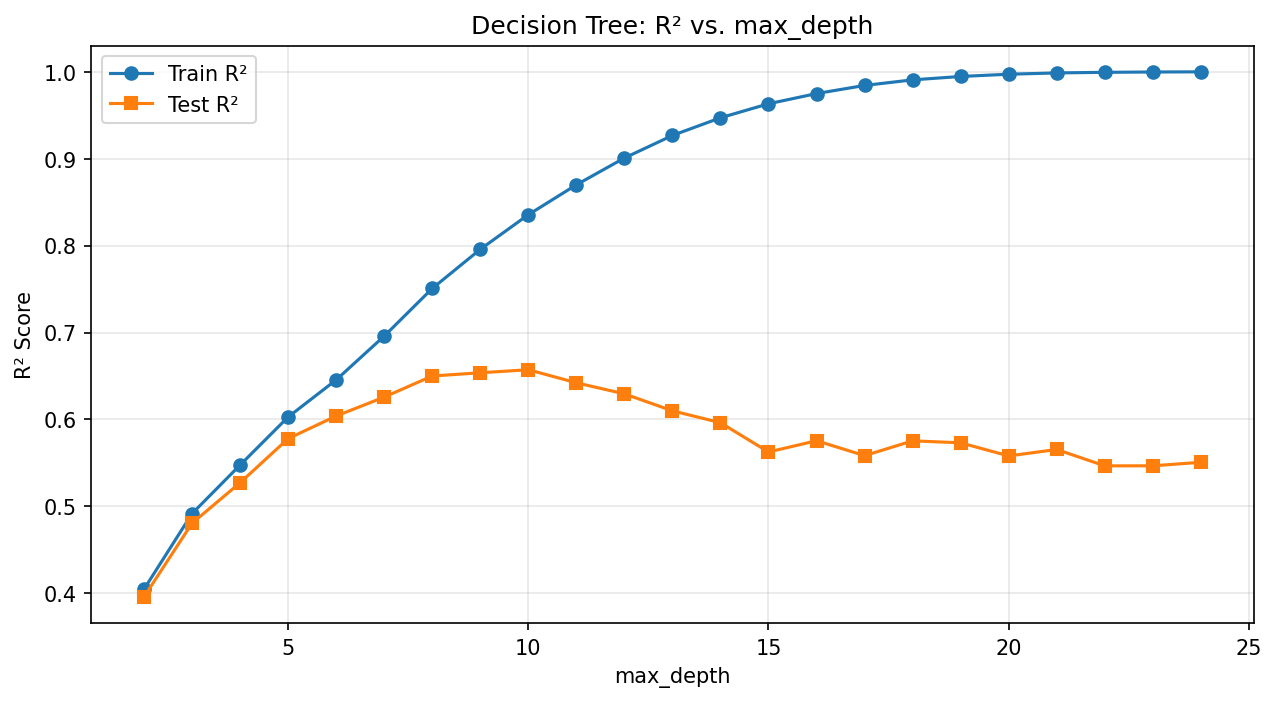
\includegraphics[width=0.85\columnwidth]{figures/dt_depth_tuning.png}
    		\caption{maximale Tiefe}
    		\label{fig:figure_3}
    	    \end{figure}

            \subsubsection{Regularisierung (Kolja)}
            Untersuchungen des Einflusses einer L2-Regularisierung verglichen mit dem Basismodell 
            ohne Regularisierung erzielte einen signifikant geringeres Overfitting-Gap (-40\%).
            Damit erbessert sich die Generalisierungsfähigkeit der Modelle erheblich. 
            Nach Analyse der L2-Regularisierung, des Dropout-Verfahrens und einer Kombination konnte ein von Modell zu Modell
            sukzessive verringertes Overfitting zulasten des $R^2$ festgestellt werden.
            Durch die drastische Verringung des Overfittinggaps reduzierte sich dieser um einige Zehntel Prozent.

            \subsubsection{Aktivierungsfunktionen (Felix H., Kolja)}
             Ein Test der sechs gängigsten Aktivierungsfunktionen (ReLU, tanh, sigmoid, ELU, SELU, Leaky-ReLU) im Zusammenspiel mit
             den verschiedenen Skalierung zeigt die beste Leistung auf den Testdaten mit dem Tangens hyperbolicus angewandt
             auf den Standard-Scaler. Dieser erzeugt viele Daten um Null herum, die tangens hyperbolicus gut verarbeiten kann.
             Zudem neigt diese Funktion wegen ihrer Glätte zu wenig Overfitting. Spätere komplexere Modelle zeigen,
             dass die Leistung nur geringfügig von der Aktivierungsfunktion abhängt und die Wahl dem Modell überlassen werden kann.

            \subsubsection{Hyperparameter (Björn, Felix H., Felix N.)}
            Zunächst fand eine Analyse der Hyperparameter unter festhalten der restlichen Parameter statt, um eine Idee für die Größenordnung zu gewinnen.
            Die isolierte Hyperparameterbetrachtung endete dabei häufig in lokalen Minima ohne eindeutiges Optimum.
            Dennoch stellten sich folgende Größenordnungen als Anhaltspunkte für weitere Untersuchungen heraus.
            \begin{table}[H]
        	\caption{Ergebnisse der Hyperparameteruntersuchung}
        	\label{tab:table}
        	\begin{tabular}{
        		>{\raggedright\arraybackslash}p{0.25\columnwidth}
        		>{\raggedright\arraybackslash}p{0.25\columnwidth}
        		>{\raggedright\arraybackslash}p{0.40\columnwidth}
        	}
        	\toprule
        	\textbf{Hyperparameter} & \textbf{Größenordnung} & \textbf{Kommentar} \\
        	\midrule
        	Epochen            & 300-500        &                                            \\ \hline
            learning-rate      & 0.01- 0.001    & im Folgeneden meist mit Lr-Scheduler. Dennoch fast immer in diesem Bereich  \\ \hline
            Batch-Size          & 16-128         & größer würde zu einer zu langen Konvergenzzeit führen               \\
        	\bottomrule
        	\end{tabular}
        	%\tabletext{Note: The table contains data of some famous celestial objects.}
        \end{table}
            Das Zusammenspiel der Hyperparameter wurde zunächst mit Random Search und zur höheren Recheneffizienz
            mit einer Bayesschen Optimierungsfunktion durchgeführt.
            Die Learningrateoptimierung erfolgt dynamisch während des Trainings mit einem Learningrate-Scheduler.\\
        \vspace{0.25cm}

        lles in allem führt die händische Veränderung der Architektur, der Lernrate und der Epochen zunächst zwar zu kleinen Ergebnisschwankungen,
        ist aber ohne systematisches Vorgehen und Simultanoptimierung nicht zielführend. 
        Die besten Modelle variiern daher in der Zusammensetzung der Architektur, liegen aber alle in den genannten Größenordnungen.
%%% Grafik: Differenz der Leistung auf Trainings- und Testdaten als Maß des Grades an Overfitting

        \subsection{Feature engineering (Felix N., Björn, Felix H.)}
        Eine Untersuchung der Features zeigt eine deutliche Spanne an potenziellen Informationsgewinn durch die einzelnen Features.
        Daher wurde versucht die Modelle mit den wichtigsten vier bis fünf und auch nur dem wichtigsten Feature zu trainieren.
        Eine geringere Featureanzahl verringert die Komplexität des Modells und somit die Rechenzeit.
        Obgleich eine geringere Featureanzahl zu keine höheren Leistung führt,
        können Ensembles aus  Modellen die verschieden viele Features berücksichtigen dies leisten. 
        Um die Korrelation einzelner Merkmale untereinander zu nutzen wurden weitere Features aus dem Datensatz zusammengefasst. 
        Die so neu entstandenen Features sind „Bedrooms-per-Room“,  „Dist-to-SF“ und „Dist-to-LA“, 
        als Hypothese einer Preissteigerung in Abhängigkeit der relativen Nähe zu den größten Ballungsräumen,
        sowie „Lat-x-Lon“,als allgemeine geografische Einordnung. Aufgrund der Schwierigkeiten mit schiefen Verteilungen wurde
        zudem die Population in logarithmischer Form eingebracht. 
        Auch die Einführung dieser Features brachte keine nennenswerte Leistungsteigerung $(ca. 0.5\%)$ oder Fehlerminderung mit sich.
        Dennoch haben vor allem die beiden Distance-Features einen Mehrwert für das Projekt, da ihre Feature Importance realtiv hoch ist.
        Wie im Plot \figref{fig:figure_4} zu sehen, haben die Distancefeatures keine unwesentliche Feature Importance.
        Das Median Einkommen bleibt jedoch das stärkste Feature für den Datensatz.

        \begin{figure}[H]
    		\centering
    		\includegraphics[width=0.85\columnwidth]{figures/"Feature Importance (with distance features).png"}
    		\caption{Featureimportance}
    		\label{fig:figure_4}
    	\end{figure}

        Obgleich vorallem die Distance-Features keine unwesentliche Feature Importance aufweisen,
        bleibt das Median Einkommen das stärkste Feature für den Datensatz.

        \subsection{Gesamtvergleich mit der Linearen Regression}
        Der Gesamtvergleich zwischen linearer Regression und unserem stärksten Neuronalen Netz zeigt eine deutliche Leistungsdifferenz:
         \begin{table}[H]
        	\caption{Vergleich linearer Regression mit Neuronalem Netz }
        	\label{tab:table}
        	\begin{tabular}{
        		>{\raggedright\arraybackslash}p{0.2\columnwidth}
        		>{\raggedright\arraybackslash}p{0.28\columnwidth}
        		>{\raggedright\arraybackslash}p{0.4\columnwidth}
        	}
        	\toprule
        	\textbf{Metrik} & \textbf{Lineare Regression} & \textbf{Neuronales Netz} \\
        	\midrule
        	$R^2-Score$        & 0.6326  &  0.7958 ($\Delta_{Baseline} R^2 = 0.1632$)       \\
            MAE                & 0.4331  &  0.2895       \\
            RMSE               & 0.5779  &  0.4308        \\
        	\bottomrule
        	\end{tabular}
        	%\tabletext{Note: The table contains data of some famous celestial objects.}
        \end{table}

        Der direkte Vergleich zwischen linearer Regression und neuronalen Netzen 
        offenbart ein klassisches Spannungsfeld in der Datenwissenschaft: die Abwägung zwischen Vorhersagegenauigkeit und Interpretierbarkeit.
        Da bereits ein einfaches neuronales Netz als Minimalnetz einen deutlich besseren Score auf den Testdaten 
        erzielt als die lineare Regression vgl. \figref{fig:figure_5},
        lässt sich schließen, dass die Features und ihr Zusammenwirken komplexe, nichtlineare Zusammenhänge aufweisen.
        Während neuronale Netze diese abbilden können, bedarf es bei der linearen Regression aufwendigen
        Feature-Engineering, wie etwa durch polynomiale Erweiterungen. 
        
        \begin{figure}[H]
    		\centering
    		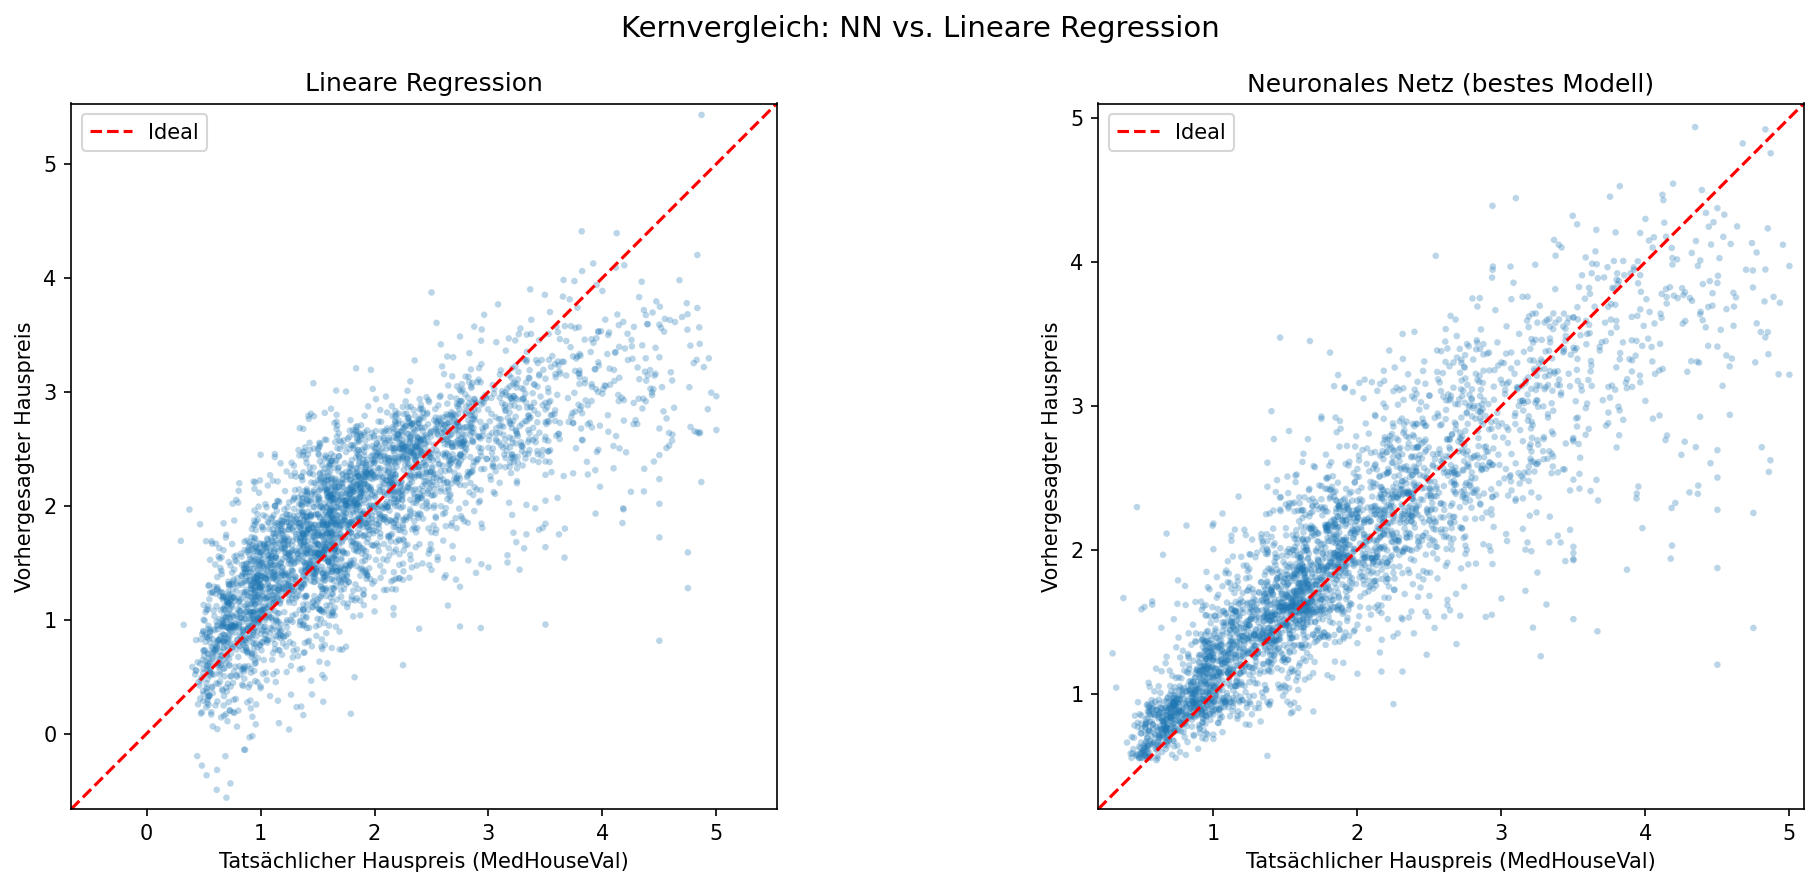
\includegraphics[width=0.85\columnwidth]{figures/nn_vs_linear_regression.png}
    		\caption{Lineare Regression vgl. einfaches Neuronales Netz}
    		\label{fig:figure_5}
    	\end{figure}

    
        Das Training eines NN benötigt ein Vielfaches an Rechenzeit und benötigt ein umfangreiches Hyperparameter-Tuning,
        unter anderem bezüglich der Architektur, Lernrate, Dropout-Rate und Batch-Größe für ein optimales Ergebnis.
        Wie die Untersuchungen zeigten, neigt beispielsweise ein unreguliertes Modell mit einer
        [128-64-32]-Neuronenverteilung zu starkem Overfitting.
        Die Generalisierungsfähigkeit kann jedoch durch den Einsatz von Regularisierung und Dropout erheblich robuster
        gestaltet werden.

        Zudem fehlt den neuronalen Netzen die Interpretierbarkeit fast vollständig.
        Die lineare Regression hingegen überzeugt durch ihre leicht nachvollziehbaren Koeffizienten.

        Die nicht-linearen Zusammenhänge des kalifornischen Hauspreis Datensatzes lassen sich sehr gut 
        durch ein neuronales Netz beschreiben. Das Optimalergebnis des Random Forest mit Gradient Boosting wurde jedoch noch nicht erreicht.
        Mögliche Ansätze für noch weitere Optimierungen wäre zum Beispiel der Einsatz von Batch Normalization zur
        Stabilisierung des Lernprozesses oder die Verwendung eines Powertransformers. Ansätze wie die bereits untersuchte manuelle
        Logarithmisierung der Population könnten damit automatisiert werden. Dass dies zu Lasten der Interpretierbarkeit geht,
        wöge im Vergleich zur linearen Regression nicht weiter auf. 

        
        




\begin{comment}


\section{Document Styling}

    \subsection{Document Type}

        Before the main title, a brief descriptor indicates the type of document (e.g., Lab Report, Research Article, etc). This is controlled by the \inlinecode{\doctype{}} command. 
        
        If no such label is needed, omit the command and the title will automatically reposition itself to maintain proper vertical spacing and visual alignment.

    \subsection{Abstract and Keywords}

        The abstract and keywords are declared in the preamble of the document, before the beginning of the document, and are automatically positioned during the title creation process.

    \subsection{Lettrine}

		The \inlinecode{\taustart{}} command, provides a personalized lettrine for the beginning of the first paragraph as shown in this example.

	\subsection{Table of Contents}

        This class includes a customized design for the table of contents, which is disabled by default. To enable it, insert the \inlinecode{\tableofcontents} command before your first section.

    \section{Cross-Reference Commands*}

        Tau-class provides shorthand commands for cross-referencing figures, tables, code listings, and equations. To customize the label format, edit the \inlinecode{taubabel.sty} file. Label translations for Spanish are handled automatically.

        \begin{itemize}
            \item \inlinecode{\figref{}} — Uses the label style defined by \inlinecode{\figlabel}.
            \item \inlinecode{\figsref{}} — Uses the label style defined by \inlinecode{\figslabel}.
            \item \inlinecode{\tabref{}} — Uses the label style defined by \inlinecode{\tablabel}.
            \item \inlinecode{\coderef{}}  — Uses the label style defined by \inlinecode{\captionlabelcode}.
            \item \inlinecode{\equref{}} — Uses the label style defined by \inlinecode{\eqlabel}.
        \end{itemize}
        
         These commands generate fully hyperlinked references, both the label and the number, ensuring navigation to the referenced element when clicked in the PDF.

\section{Figures and Tables}

    \subsection{Figures}
		
    	\figref{fig:figure} shows a 3D surface plot of the hyperbolic paraboloid $z=x^2-y^2$.
    		
    	\begin{figure}[H]
    		\centering
    		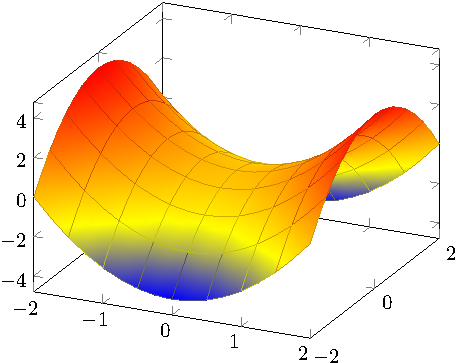
\includegraphics[width=0.75\columnwidth]{figures/Example.pdf}
    		\caption{Hyperbolic paraboloid obtained from PGFPlots \cite{PFGPlots}.}
    		\label{fig:figure}
    	\end{figure}

    \subsection{Tables}
	
        \tabref{tab:table} shows an example table of some astronomical objects. 

        \begin{table}[H]
        	\caption{Astronomical Object Data}
        	\label{tab:table}
        	\begin{tabular}{
        		>{\raggedright\arraybackslash}p{0.25\columnwidth}
        		>{\raggedright\arraybackslash}p{0.30\columnwidth}
        		>{\raggedright\arraybackslash}p{0.31\columnwidth}
        	}
        	\toprule
        	\textbf{Object} & \textbf{Type} & \textbf{Distance (Light Years)} \\
        	\midrule
        	Alpha Centauri & Star system & 4.37 \\
        	Betelgeuse & Red supergiant star & 642.5 \\
        	Andromeda & Spiral galaxy & 2.537 million \\
        	Earth & Planet & 0 \\
        	Sirius & Binary star system & 8.6 \\
        	\bottomrule
        	\end{tabular}
        	\tabletext{Note: The table contains data of some famous celestial objects.}
        \end{table}

        The \inlinecode{\tabletext{}} command is used to add notes to tables easily. 

\section{Document Data}

    \subsection{Front-Matter Footer Block*}

        The \inlinecode{\docinfo{}} command inserts a dedicated block at the bottom of the first column. Unlike floating elements, this block stays fixed in place — positioned visually like a footnote, although technically it is not one.
    
        The \inlinecode{\docinfo{}} block was created to give you greater control over supplementary document data, such as publication dates, licensing information, extended author details, and other front-matter notes. You can fully customize its content to suit your needs. If it’s not required, omit the command to remove this block entirely.
    
        \begin{note}
            This feature has been adapted to work seamlessly alongside the standard \verb|\thanks{}| command, which is commonly used to indicate corresponding authors, equal contributions, or other acknowledgments.
        \end{note}
    
        If \inlinecode{\thanks{}} is not used, \inlinecode{\docinfo{}} will automatically adjust its position. The implementation was designed to handle any combination of front-matter elements you might need when starting your document. In this example template, you’ll find a minimal demonstration that combines both to illustrate their interaction.

    \subsection{Headers and Footers}

        \subsubsection{Headers}

            On all pages except the first, the document title appear in the header. Since twoside layout is enabled, its position alternates depending on whether the page is odd or even.

        \subsubsection{Footers}

            On odd-numbered pages, five elements display supplementary information for your document:
    
            \begin{itemize}
                \item \inlinecode{\thepage} — Including the total number of pages (only for the first page).
                \item \inlinecode{\footinfo{}} — For a short title or custom note.
                \item \inlinecode{\theday{}} — Displays the current date.
                \item \inlinecode{\organization{}} — For a university, institute, company, or any institutional affiliation.
                \item \inlinecode{\leadauthor{}} — For the main author name et al.
            \end{itemize}

            On even-numbered pages, the page number appears alongside the content of \inlinecode{\footinfo{}} and, on the other side, the \inlinecode{\leadauthor{}}. 

            In contrast to the header, the footer elements do not alternate their positions. The footer is explicitly configured for either odd or even pages, resulting in a fixed layout.
            
            In all cases, you can freely rearrange or customize the order of these elements by modifying the class file to suit your needs. If any of them are not required, simply omit the corresponding command — the remaining elements will automatically adjust their spacing to remain evenly distributed.

\section{Tau Custom Packages}

    \subsection{Taubabel.sty}
		
		This package have all the commands that automatically translate from English to Spanish when this custom package is defined. 
		
		By default, this document has its content in English. However, at the beginning of the document you will find a recommendation when writing in Spanish. 
		
		You may modify this package if you want to use other language than English or Spanish. This will make easier to translate your document without having to modify the class document.

	\subsection{Tauenvs.sty}

        This package provides custom environments designed to enhance the visual presentation and structure of your document. Key examples include tauenv, info, and note.
        
		Their style is defined by \inlinecode{tauenvstyle} — allowing you to customize their appearance according to your document’s requirements.

		An example using the \inlinecode{tauenv} environment is shown below.
		
		\begin{tauenv}[frametitle=Custom Title]
			This is an example of the custom title environment. To add a title type this command \verb|[frametitle=Custom Title]| next to the beginning of thie environment (as shown in this example).
		\end{tauenv}

        The \inlinecode{info} and \inlinecode{note} are environments which have a predefined title and translate their title to Spanish automatically when this language is defined.

\section{Equations}

	\equref{eq:equation} shows the Schrödinger equation as an example. 

    \begin{equation}\label{eq:equation}
        i\hbar \frac{\partial }{\partial t}\Psi(\mathbf{r},t) = \left[\frac{-\hbar^2}{2m}\nabla^2 + V(\mathbf{r},t) \right]\Psi(\mathbf{r},t)
    \end{equation}
	
	The \inlinecode{amssymb} and \inlinecode{amsmath} packages were not required, as \href{https://ctan.org/pkg/stix2-otf/}{STIX2} font incorporates mathematical symbols for writing quality equations.
	
	\begin{note}
		If you would like to change the values that adjust the spacing above and below the equations, change the \verb|\eqskip| value until the preferred spacing is set. The default value is set to 9pt.
	\end{note}

\section{Codes}

	\subsection{Coding with Minted*}
	
		The \inlinecode{minted} package offers customized features for adding codes. In addition, the template is designed to work seamlessly with Fira Code, a monospaced font specially crafted for programming environments.

        If your are using a desktop app as \href{https://www.texstudio.org/}{TeXstudio}, try these steps to make this package work on Windows:
		
		\begin{enumerate}
			\item Install Python — A stable version (e.g., v.3.11)
			\item Open the terminal and type \inlinecode{pip install Pygments}.
			\item Update if a newer version is available.
			\item Go to TeXStudio settings and change the default compiler to \inlinecode{pdflatex --shell-escape -interaction=nonstopmode \%.tex}.
			\item Compile and wait for the result.
		\end{enumerate}
        
		\vspace*{-9pt}
        
		\begin{tauenv}[frametitle=Caution]
			Ensure that \textbf{pygments} is properly installed and added to your system’s PATH. Otherwise, you may encounter compilation errors. Additionally, enable shell escape when compiling, as it is required for minted to process and highlight code.
		\end{tauenv}
		
		In Overleaf, this package is easier to use since it does not require any additional installations or modifications — just add the code as shown in the example. \coderef{lst:example} shows a Python example.
		
		\begin{code}
			% \inputminted{python}{example.py}
            \caption{Python code example with minted.}
			\label{lst:example}
		\end{code}
		
		You can customize its design changing \inlinecode{\usemintedstyle} command. The different styles offered by the \href{https://ctan.org/pkg/minted}{minted package} can be preview through this link — \url{https://pygments.org/styles/}.

    \subsection{Coding with Listings}
	
		Since \inlinecode{minted} requires additional installations and can be complex in some desktop \TeX\ editors, you can use the \inlinecode{listings} package instead, which provides a simpler way to include code.
		
		\begin{code}
			\lstinputlisting[language=python]{example.py}
			\label{lst:example2}
            \caption{Python code example with listings.}
		\end{code}
		
		While \inlinecode{listings} is a simpler and widely supported package for code formatting, \inlinecode{minted} offers a more modern and powerful approach. It leverages the Pygments syntax highlighter to deliver superior coloring, language support, and styling options. One of its key advantages is the ability to easily switch between built-in color styles.
		
		In contrast, \inlinecode{listings} requires manual setup for colors, fonts, and formatting rules.
		For users who prefer fine-tuned customization, the styling options for \inlinecode{listings} are organized in \inlinecode{tau.cls} file and can be modified at any time to suit individual preferences.

	\subsection{Inline Code*}
	
		As shown in this template, inline code has a custom style for improved visual appeal. To use it, simply add \inlinecode{\inlinecode{}} command and place your code inside the braces.

\section{Bibliography}
		
	Bibliography management is handled by \inlinecode{biblatex}, with the default citation and reference style set to IEEE. The \inlinecode{citestyle=numeric-comp} option is enabled, allowing multiple citations to be grouped within a single bracket (e.g., \cite{davis2023signalflow,bell2022codefont}). The citation format can be customized directly in \inlinecode{tau.cls} to suit any preferred style.

\section{FAQ}

    \subsection*{How do I manage my references?}
        
        To manage your references, I recommend using the tool \href{https://www.scribbr.es/citar/generador/folders/73QOXYsCwMRu4ifQaN65mx/lists/msTfx7GJjIAOUkufbISnA/}{scribbr}. You can simply enter the URL or create your own citation, and then export it to \LaTeX\ using the options in the three-dot menu.
            
        The generated citation can be copied and pasted into \inlinecode{tau.bib}, the file designated for bibliography management. You may rename this file, but if you do, remember to update the \inlinecode{\addbibresource} command in \inlinecode{tau.cls} under the biblatex section.
    
        \begin{note}
            Some platforms, such as Google Scholar or scientific journals, provide citations directly in BibTeX format. Therefore, check if there is a ``how to cite this document'' section to streamline the citation process even further.
        \end{note}

        If you have any further questions, you can refer to the following page — \href{https://es.overleaf.com/learn/latex/Bibliography_management_with_biblatex}{Bibliography management with biblatex}.
        
    \subsection*{What should I do with the example files?}

        The template includes sample content — such as an example figure, bibliography entries, and the \inlinecode{example.py} script — to demonstrate how the layout and features work. Once you start customizing the document for your own use, feel free to delete all example files and entries you don’t need.

    \subsection*{How do I place equations easily?}

        For equations, we have two options: inline or on its own line. For inline equations, simply place a dollar sign (\$) at the beginning and end of the equation. However, if you want the equation to be displayed on its own line, you need to use the equation environment.
        
        If you find it challenging to write formulas directly in \LaTeX, you can use text editors like Word. In the equations menu, you can select \LaTeX\ in the conversion section and copy and paste the equation you wrote into one of these two environments.

    \subsection*{How do I change the paper size?}

        By default, this class was adapted for a4paper and test it with letterpaper. The following paper sizes are available in \LaTeX:

        \begin{itemize}
            \item letterpaper (11 $\times$ 8.5 in)
            \item legalpaper (14 $\times$ 8.5 in)
            \item executivepaper (10.5 $\times$ 7.25 in)
            \item a4paper (21 $\times$ 29.7 cm)
            \item a5paper (21 $\times$ 14.8 cm)
            \item b5paper (25 $\times$ 17.6 cm)
       \end{itemize}

\section*{Contact me}
    
    Have questions, suggestions, or an idea for a new feature? Found a bug or working on a project you’d like to invite me to?  
    
    Feel free to reach out — I’d be happy to help, collaborate, or fix the issue.  Your feedback helps me improve my templates!

    \AtBeginEnvironment{tabular}{\normalsize\sffamily\selectfont}
    \begin{center}
        \setlength{\tabcolsep}{3pt}
        \begin{tabular}{cl}
            \faEnvelope & \href{mailto:memo.notess1@gmail.com}{memo.notess1@gmail.com} \\
            \faGlobe{} & \href{https://memonotess1.wixsite.com/memonotess}{memonotess.com} \\
            \faInstagram{} & \href{https://www.instagram.com/memo.notess/}{@memo.notess}
        \end{tabular}
    \end{center}

\section*{Github Repository}

    Visit the repository to access the source code, track ongoing development, report issues, and stay up to date with the latest changes.

    \begin{center}
        \setlength{\tabcolsep}{3pt}
        \begin{tabular}{cl}
             \faGithub &  \url{https://github.com/MemoJimenez/Tau-class}\\
        \end{tabular}
    \end{center}

\section*{Supporting}

    Did you like this class document? Check out rho-class, made for complex research articles.

    \begin{center}
        \setlength{\tabcolsep}{3pt}
        \begin{tabular}{cl}
             \faLink &  \href{https://es.overleaf.com/latex/templates/rho-class-academic-article-template/bpgjxjjqhtfy}{https://es.overleaf.com/latex/templates/rho-class}\\
        \end{tabular}
    \end{center}
    
    \subsection*{Any contributions are welcome!}
    
        Coffee keeps me awake and helps me create better \LaTeX\ templates. If you wish to support my work, you can do so through PayPal: 

        \begin{center}
            \setlength{\tabcolsep}{3pt}
            \begin{tabular}{cl}
                 \faPaypal & \textbf{\url{https://www.paypal.me/GuillermoJimeenez}}\\
            \end{tabular}
            \vskip9pt
            Enjoy writing with tau-class!
        \end{center}
\end{comment}
%----------------------------------------------------------

\printbibliography

%----------------------------------------------------------

\end{document}